\documentclass[12pt,a4paper,oneside]{report}
\usepackage{indentfirst}
\usepackage{times}
\usepackage[ddmmyyyy,hhmmss]{datetime}
\setlength\parindent{1cm}
\renewcommand{\baselinestretch}{1.50}\normalsize
\usepackage{anysize}
\marginsize{1.25in}{.75in}{1in}{1in}
\usepackage{graphics}
\usepackage{graphicx}
\usepackage{epsfig}
\usepackage[fleqn]{amsmath}
\usepackage{amsfonts}
\usepackage{textcomp}
\usepackage{graphicx}
\usepackage{setspace}
\usepackage{fancyhdr}
\usepackage{truncate}
\usepackage{nomencl} 
\usepackage{acronym}
\usepackage{array}
\usepackage{caption}\usepackage{subcaption}
\usepackage{subfig}
\usepackage[overload]{textcase}
\usepackage{listings}
\renewcommand{\nomname}{List of Abbreviations}
\usepackage{makeidx}
\makeindex
\makenomenclature
\newcommand{\quotes}[1]{``#1''}
\usepackage{titlesec}
\titleformat{\chapter}[display]
{\normalfont\Large\bfseries\centering}
{\chaptertitlename\ \thechapter}{15pt}{\LARGE}
\titleformat{\section}{\large\bfseries}{\thesection}{1em}{}
\titleformat{\subsection}{\normalsize\bfseries}{\thesubsection}{1em}{}
\renewcommand{\chaptermark}[1]{\markboth{ \emph{#1}}{}}

\printnomenclature[5em]
\pagestyle{fancy}
%\headheight 1pt
	\renewcommand{\footrulewidth}{1.2pt}
\renewcommand{\headrulewidth}{1.2pt}
\rhead{\scriptsize {\leftmark}}

\lhead{\small{College of Engineering, Cherthala \;\;\;\;\;\;\;\;\;\;\;\;\;\;\;\;\;\;}}
\rfoot{\thepage}
\cfoot{\empty}
\lfoot{\small{Department of Computer Science \& Engineering}}
%\renewcommand{\figurename}{Fig.}
\begin{document}
\renewcommand\bibname{References}
\begin{titlepage}
\begin{center}
\Large{\textbf{MAJOR PROJECT REPORT}}\\
\vspace{.2 in}
\begin{singlespace}
\LARGE{\textbf{Continuous Integration Pipeline Implementation for Tech11Software }}\\
\end{singlespace}
\vspace{.2 in}
\Large{\textit{Submitted By }}\\
\Large{\textit{\textbf{ASWIN G SUGUNAN }\textbf{(Reg.No . 121436--)}}} \\
\Large{\textit{\textbf{JEFFIN JACOB  }\textbf{(Reg.No . 12143611)}}} \\
\Large{\textit{\textbf{NITIN SURESH }\textbf{(Reg.No . 121436--)}}} \\
\Large{\textit{\textbf{VISHNU BOSE }\textbf{(Reg.No . 121436--)}}} \\
\Large{\textit{\textit{under the guidance of}}}\\
\Large{\textit{\textbf{Mrs. GREESHMA N GOPAL}}}\\
\Large{\textit{(Assistant Professor)}}\\
\Large{\textit{(Computer Science \& Engineering)}}
\vspace{.05in}
\begin{figure}[h]
\begin{center}

\epsfig{width=1 in, file=logo.jpg}
\end{center}
\end{figure}
\begin{singlespace}
\large{\textbf{MARCH 2017}}\\
\vspace{.1in}
\large{\textbf{DEPARTMENT OF COMPUTER SCIENCE AND ENGINEERING\\COLLEGE OF ENGINEERING,CHERTHALA\\ PALLIPPURAM P O, ALAPPUZHA-688541, \\PHONE: 0478 2553416, FAX: 0478 2552714\\http://www.cectl.ac.in}}
\end{singlespace}
\end{center}
\end{titlepage}
\begin{titlepage}
\begin{center}

\large{\textbf{MAJOR PROJECT REPORT}}\\

\LARGE{\textbf{Continuous Integration Pipeline Implementation for Tech11Software}}\\

\Large{\textit{Submitted By }}\\
\begin{singlespace}
%\begin{singlespace}
\Large{\textit{\textbf{ASWIN G SUGUNAN }\textbf{(Reg.No . 121436--)}}} \\
\Large{\textit{\textbf{JEFFIN JACOB  }\textbf{(Reg.No . 12143611)}}} \\
\Large{\textit{\textbf{NITIN SURESH }\textbf{(Reg.No . 121436--)}}} \\
\Large{\textit{\textbf{VISHNU BOSE }\textbf{(Reg.No . 121436--)}}} \\

\end{singlespace}
\Large{\textit{\textit{under the guidance of}}}\\
\Large{\textit{\textbf{Mrs. GREESHMA N GOPAL}}}\\
\begin{singlespace}
\small{\textit{In partial fulfilment of the requirements for the award of the degree}\\
\small{ \textit{of}}\\
\small{\textit{Bachelor of Technology} }\\
\small{\textit{in}}\\
\small{\textit{Computer Science and Engineering}}\\
\small{\textit{of}}\\
\small{\textit{Cochin University Of Science And Technology}}}\\
\end{singlespace}
\begin{singlespace}
\begin{figure}[h]
\begin{center}

\epsfig{width=1 in, file=logo.jpg}
\end{center}
\end{figure}
\end{singlespace}
\begin{singlespace}

\Large{{\textbf{MARCH 2017\\Department of Computer Science and Engineering\\College of Engineering, Cherthala}\\
Pallippuram P O, Alappuzha-688541 \\Phone: 0478 2553416, Fax: 0478 2552714}}
\end{singlespace}
\end{center}
\end{titlepage}
\begin{titlepage}
\begin{center}

\large{\textbf{DEPARTMENT OF COMPUTER SCIENCE \& ENGINEERING}}\\
\large{\textbf{COLLEGE OF ENGINEERING CHERTHALA\\ALAPPUZHA-688541}}\\
\end{center}
\begin{figure}[h]
\begin{center}

\epsfig{width=1.5in, file=logo.jpg}
\end{center}
\end{figure}
\begin{center}
\large{\textbf{C E R T I F I C A T E}}\\
\end{center}
\begin{spacing}{1.5}
This is to certify that, the major project report submitted by \newline Name: \hspace{300pt} Date:\today\newline Reg.No:\newline
On \textbf{\textit{Continuous Integration Pipeline Implementation for Tech11Software}}
 in partial fulfillment of the requirements for the award of the degree, \textbf{B. Tech. Computer Science  \& Engineering } of \textbf{Cochin University of Science \& Technology}.
\end{spacing}
\begin{tabbing}
xxxxxxxxxxxxxxxxxxxxxxxxxxxxxxxxxxxxxx\= xxxxxxxxxxxxxxxxxxxx\= \kill
\hspace{.15in}{\bf Guide} \>\hspace{-.7in}{\bf Co-ordinator}\hspace{1.45in}{\bf  HoD  } \\
\end{tabbing}
\begin{tabbing}
xxxxxxxxxxxxxxxxxxxxxxxxxxxxxxxxxxxxxx\= xxxxxxxxxxxxxxxxxx\= \kill
%\vspace{0.3in}\\
\hspace{.15in}{\bf{Mrs. Greeshma N Gopal K}}   \>\hspace{-.7in}{\bf Mrs. Sreelakshmi Murali} \hspace{.55 in}{\bf Dr. Preetha Theresa Joy}\\
\hspace{.15in}Assistant Professor    \>\hspace{-.7in}Assistant Professor\>\hspace{.20in}Professor\\
\hspace{.1in} Computer Science\&Engg    \>\hspace{-.75in}    Computer Science\&Engg \>\hspace{.15in}    Computer Science\&Engg\\

\end{tabbing}
\end{titlepage}


\renewcommand*\thesection{\thechapter.\arabic{section}}
%\pagenumbering{arabic}
%\addtocounter{page}{4}


\begin{titlepage}
\pagenumbering{arabic}
%\addtocounter{page}{4}
\setcounter{page}{4}
\section*{\begin{center} \Large{ACKNOWLEDGEMENT }\end{center}}

\thispagestyle{plain}


%{$\;\;\;\:$}
\par
We take this opportunity to express our sincere gratitude to the people who have been
instrumental in the successful completion of our major project.
For every endeavour in our life, the help of the Lord has always followed. We have yet
again experienced his loving kindness while preparing for this project.
We would like to express our sincere thanks to the Principal, \textbf{Dr. Mini M. G}, for her
valuable support and advice. We would also like to thank our Head Of Computer Science
Department, \textbf{Dr.Preetha Teresa Joy} (Professor, Computer Science and Engineering Department) for her support. We express our heartfelt gratitude to
our project coordinator, \textbf{Mrs. Sreelakshmi Murali} (Assistant Professor, Computer Science and Engineering Department) for her valuable help and support. We would also like to thank our project Guide,
\textbf{Mrs. Greeshma N Gopal} (Assistant Professor, Department of Computer Science) for her support and
guidance.
We are indebted to all teaching and non-teaching staff of the Department of Computer
Science and Engineering, friends and family for their co-operation and support, with out which
we could never have completed the project this well. \\
\end{titlepage}
\newpage

\section*{\begin{center}\Large ABSTRACT\end{center}}
\thispagestyle{empty}
\par
\hspace{0.1in}
{
Software development, as we know it today, is a demanding area of business with its fast-changing customer requirements, pressures of an ever shorter timeto- market, and unpredictability of market. With the shift towards modern continuous deployment pipelines, releasing new software versions early and often has become a concrete option also for an ever growing number of practitioners. \par Continuous delivery is a software development practice where new features are made available to end users as soon as they have been implemented and tested. In such a setting, a key technical piece of infrastructure is the development pipeline that consists of various tools and databases, where features ow from development to deployment and then further to use.
\tableofcontents
\pagenumbering{roman}
\listoffigures


\def\addsymbol #1: #2#3{\;\;\;\;\;\;\;\;\;\;\;\;\;\;\;\;\;\;\;\;\;\;\;$#1$ \> \;\;\;\;\;\;\;\;\;\;\;\;\;\;\;\;\;\;\;\;\;\;\;\;\;\; \parbox{5in}{#2}\\}


\renewcommand*\thesection{\thechapter.\arabic{section}}
\newpage
\pagestyle{fancy}
\headheight 26pt
\renewcommand{\footrulewidth}{1.2pt}
\renewcommand{\headrulewidth}{1.2pt}
\rhead{\scriptsize {\leftmark}}
%\chead{Middle top}
\lhead{\small{College of Engineering, Cherthala \;\;\;\;\;\;\;\;\;\;\;\;\;\;\;\;\;\;}}
\rfoot{\thepage}
\cfoot{\empty}
\lfoot{\small{Department of Computer Science \& Engineering}}


\chapter{INTRODUCTION}
\label{intro}
\pagenumbering{arabic}
\setcounter{page}{1}
%\hspace{0.1in}
Software development, as we know it today, is a demanding area of business
with its fast-changing customer requirements, pressures of an ever shorter timeto-
market, and unpredictability of market. With the shift towards modern continuous deployment
pipelines, releasing new software versions early and often has become a concrete
option also for an ever growing number of practitioners. 
\par
Continuous delivery is a software development practice where
new features are made available to end users as soon as they have been
implemented and tested. In such a setting, a key technical piece of infrastructure
is the development pipeline that consists of various tools
and databases, where features 
ow from development to deployment and
then further to use.
\section{PURPOSE}
\par The objective of the project is to put in place a Continues Integration framework for product
development activities of Tech11 Software.This would enable the Tech11 team to rapidly bring a
product change or feature to production gaining market advantage.
\par
This activities of this project will involve accessing different CI integration approaches and
solutions available,identify the feasibility of those solution by doing POCs and demos,fine tune the
final solution and set up the CI infrastructures,educate the developers on CI culture.

\section{PRODUCT SCOPE}
\par  The scope of the system is to help software developers to ensure new features are made available as soon as the program has been
implemented and tested. This product also helps in reducing the time needed to develop a software and also acts a guideline for future software developments
\\

\chapter{OVERALL DESCRIPTION}
\section{PRODUCT PERSPECTIVE}
\par
Continuous Integration is based on continuous performance of acts of integration of
source code, testing, building and deployment in response to each change to the source code of
the project submitted by the developer and for the use of tools for support of the development
and testing by compliance with the established procedure automatically. The proposed system
directs the user (developers) for time and cost effective production and solves majority of the
Integration hell problem. \par
Integration Hell refers to the point in production when members on a delivery team integrate
their individual code. In traditional software development environments, this integration
process is rarely smooth and seamless, instead resulting in hours or perhaps days of fixing the
code so that it can finally integrate. Continuous Integration (CI) aims to avoid this completely
by enabling and encouraging team members to integrate frequently (e.g., hourly, or at least
daily).
%\subsection{Current system}
%\par

\subsection{Proposed System}
\par 
The Proposed system is to help software developers to ensure new features are made
available as soon as the program has been implemented and tested. This product also helps in
reducing the time needed to develop a software and also acts a guideline for future software
developments.
\section{SOLUTION FUNCTION}

\par Continuous integration – the practice of frequently integrating one's new or changed code with the existing code repository – should occur frequently enough that no intervening window remains between commit and build, and such that no errors can arise without developers noticing them and correcting them immediately.[9] Normal practice is to trigger these builds by every commit to a repository, rather than a periodically scheduled build. The practicalities of doing this in a multi-developer environment of rapid commits are such that it is usual to trigger a short time after each commit, then to start a build when either this timer expires, or after a rather longer interval since the last build. Many automated tools offer this scheduling automatically.

\begin{itemize}
\item \textbf{Version Control}

\par This practice advocates the use of a revision control system for the project's source code. All artefacts required to build the project should be placed in the repository. In this practice and in the revision control community, the convention is that the system should be buildable from a fresh checkout and not require additional dependencies.  Extreme Programming  mentions that where branching is supported by tools, its use should be minimised.[9] Instead, it is preferred for changes to be integrated rather than for multiple versions of the software to be maintained simultaneously. 
\item \textbf{Artifact Manager}
\par 
While many developers have adopted Maven as a build tool, most have yet to understand the importance of maintaining a repository manager both to proxy remote repositories and to manage and distribute software artifacts. A repository stores two types of artifacts: releases and snapshots. Release repositories are for stable, static release artifacts and snapshot repositories are frequently updated repositories that store binary software artifacts from projects under constant development. While it is possible to create a repository which serves both release and snapshot artifacts, repositories are usually segmented into release or snapshot repositories serving different consumers and maintaining different standards and procedures for deploying artifacts. Much like the difference between a production network and a staging network, a release repository is considered a production network and a snapshot repository is more like a development or a testing network. While there is a higher level of procedure and ceremony associated with deploying to a release repository, snapshot artifacts can be deployed and changed frequently without regard for stability and repeatability concerns.
\item \textbf{Continuous Integration Handler}
\par While there are many tools, I will focus on one of the most popular, Jenkins CI. This is one of the more popular (open source) tools available. Jenkins CI (the continuation of a product formerly called Hudson) allows continuous integration builds in the following ways:
\begin{itemize}
\item It integrates with popular build tools (ant, maven, make) so that it can run the appropriate build scripts to compile, test and package within an environment that closely matches what will be the production environment
\item It integrates with version control tools, including Subversion, so that different projects can be set up depending on projection location within the trunk.
\item It can be configured to trigger builds automatically by time and/or changeset. (i.e., if a new changeset is detected in the Subversion repository for the project, a new build is triggered.)
\item It reports on build status. If the build is broken, it can be configured to alert individuals by email.
\end{itemize}


Jenkins is an automation engine with an unparalleled plugin ecosystem to support all of your favorite tools in your delivery pipelines, whether your goal is continuous integration, automated testing, or continuous delivery. 
 \item  \textbf{Test Automator}
\par In software testing, test automation is the use of special software (separate from the software being tested) to control the execution of tests and the comparison of actual outcomes with predicted outcomes.[1] Test automation can automate some repetitive but necessary tasks in a formalized testing process already in place, or perform additional testing that would be difficult to do manually. Test automation is critical for continuous delivery and continuous testing. There are many approaches to test automation, however below are the general approaches used widely:

\begin{itemize}
\item Graphical user interface testing. A testing framework that generates user interface events such as keystrokes and mouse clicks, and observes the changes that result in the user interface, to validate that the observable behavior of the program is correct.
\item API driven testing. A testing framework that uses a programming interface to the application to validate the behaviour under test. Typically API driven testing bypasses application user interface altogether. It can also be testing public (usually) interfaces to classes, modules or libraries are tested with a variety of input arguments to validate that the results that are returned are correct.
\end{itemize}


\item \textbf{Continouos Deployment}
\par Continuous deployment is the next step of continuous delivery: Every change that passes the automated tests is deployed to production automatically. Continuous deployment should be the goal of most companies that are not constrained by regulatory or other requirements.

\end{itemize}

 
\section{OPERATING ENVIRONMENT}
The system is expected to be operated in Linux as well as in windows with the support of
respective JRE (Java Runtime Environment). This system based project is completely platform
independent. The most important requirement is the Internet connection. This tool is coded
using JDK 1.6.
\section{GANTT CHART} 
\par Gantt chart is a graphical representation of allocation of resources to the activities. Here
our resource is time. A Gantt chart is a type of bar chart that illustrates a project schedule.
Gantt charts illustrate the start and finish dates of the terminal elements and summary elements
of a project. Terminal elements and summary elements comprise the work breakdown structure
of the project. Some Gantt charts also show the dependency (i.e., precedence network)
relationships between activities.
\par Gantt charts have become a common technique for representing the phases and activities
of a project work breakdown structure (WBS), so they can be understood by a wide audience.
Although a Gantt chart is useful and valuable for small projects that fit on a single sheet or
screen, they can become quite unwieldy for projects with more than about 30 activities. Larger
Gantt charts may not be suitable for most computer displays. A related criticism is that Gantt
charts communicate relatively little information per unit area of display. That is, projects are
often considerably more complex than can be communicated effectively with a Gantt chart.
Although project management software can show schedule dependencies as lines between activities,
displaying a large number of dependencies may result in a cluttered or unreadable
chart.
\par Because the horizontal bars of a Gantt chart have a fixed height, they can misrepresent
the time-phased workload (resource requirements) of a project, which may cause confusion especially
in large projects. A related criticism is that all activities of a Gantt chart show planned
workload as constant. In practice, many activities (especially summary elements) have front loaded
or back-loaded work plans, so a Gantt chart with percent-complete shading actually may
lead to mis-communications on the true schedule performance status.
\newpage
\begin{figure}[h]
\begin{center}
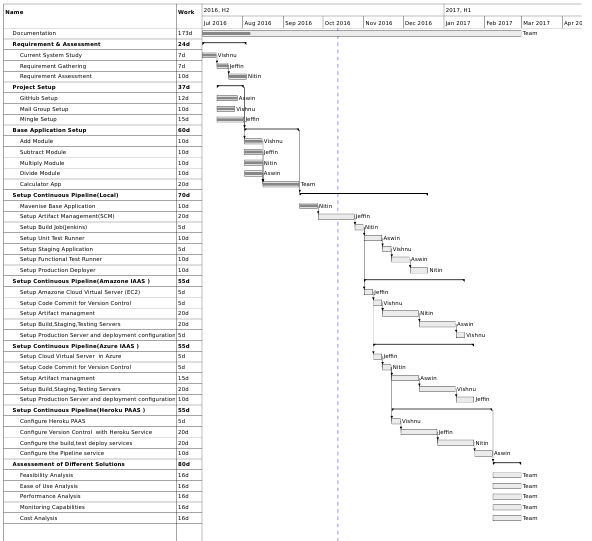
\includegraphics[scale=1]{gnt.png}
\caption{Gantt chart}
\label{Gantt chart}
\end{center}
\end{figure}
\newpage

\section{COST ESTIMATION}
\par Basic COCOMO computes software development effort (and cost) as a function of program
size. Program size is expressed in estimated thousands of lines of code (KLOC).
\par COCOMO applies to three classes of software projects:
\begin{itemize}
\item  Organic projects - “small” teams with “good” experience working with “less than rigid”
requirements.
\item Semi-detached - “medium” teams with mixed experience working with a mix of rigid
and less than rigid requirements
\item Embedded projects - developed within a set of “tight” constraints (hardware, software,
operational ...)
\end{itemize}
\par The basic COCOMO equations take the form:
\par Effort Applied = a(KLOC)\textasciicircum b [ person-months ]
\par Development Time = c(Effort Applied)\textasciicircum d [ months ]
\par People required = Effort Applied / Development Time [ count ]
\par The coefficients a, b, c and d are given in the following table.
\begin{figure}[h]
\begin{center}
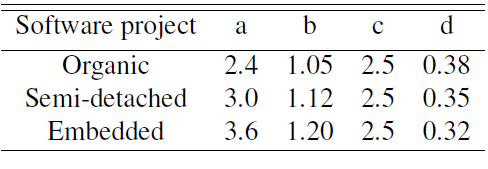
\includegraphics[scale=.6]{cocomo.PNG}
\caption{COCOMO Model Coefficients}
\label{COCOMO Model Coefficients}
\end{center}
\end{figure}
\par
\section{EXTERNAL INTERFACE REQUIREMENTS}
This system based software can be used in any operating system such as Microsoft Windows, Linux or any kind of user application interface, since it is platform independent.

\subsection{User Interface}
Interface hardware shall be encapsulated in a set of classes that isolate hardware specifications from the rest of the software. In particular, interfaces for specific hardware boards shall be implemented as derived classes of an abstract class.
\\

\subsection{Network Requirements}  
\begin{itemize}
\item Systems need minimum speed internet connection.
\end{itemize}
\subsection{Software Requirements}
\begin{itemize}
\item Git
\item Jenkins
\item Checkstyle
\item Findbugs
\item Mingle
\end{itemize}
\chapter{SYSTEM DESIGN}
\section{MODULES}
\subsection{Version Control}

\par This practice advocates the use of a revision control system for the project's source code. All artefacts required to build the project should be placed in the repository. In this practice and in the revision control community, the convention is that the system should be buildable from a fresh checkout and not require additional dependencies.  Extreme Programming  mentions that where branching is supported by tools, its use should be minimised.[9] Instead, it is preferred for changes to be integrated rather than for multiple versions of the software to be maintained simultaneously. 
\subsection{Artifact Manager}
\par 
While many developers have adopted Maven as a build tool, most have yet to understand the importance of maintaining a repository manager both to proxy remote repositories and to manage and distribute software artifacts. A repository stores two types of artifacts: releases and snapshots. Release repositories are for stable, static release artifacts and snapshot repositories are frequently updated repositories that store binary software artifacts from projects under constant development. While it is possible to create a repository which serves both release and snapshot artifacts, repositories are usually segmented into release or snapshot repositories serving different consumers and maintaining different standards and procedures for deploying artifacts. Much like the difference between a production network and a staging network, a release repository is considered a production network and a snapshot repository is more like a development or a testing network. While there is a higher level of procedure and ceremony associated with deploying to a release repository, snapshot artifacts can be deployed and changed frequently without regard for stability and repeatability concerns.
\subsection{Continuous Integration Handler}
\par While there are many tools, I will focus on one of the most popular, Jenkins CI. This is one of the more popular (open source) tools available. Jenkins CI (the continuation of a product formerly called Hudson) allows continuous integration builds in the following ways:
\begin{itemize}
\item It integrates with popular build tools (ant, maven, make) so that it can run the appropriate build scripts to compile, test and package within an environment that closely matches what will be the production environment
\item It integrates with version control tools, including Subversion, so that different projects can be set up depending on projection location within the trunk.
\item It can be configured to trigger builds automatically by time and/or changeset. (i.e., if a new changeset is detected in the Subversion repository for the project, a new build is triggered.)
\item It reports on build status. If the build is broken, it can be configured to alert individuals by email.
\end{itemize}


Jenkins is an automation engine with an unparalleled plugin ecosystem to support all of your favorite tools in your delivery pipelines, whether your goal is continuous integration, automated testing, or continuous delivery. 
\subsection{Test Automator}
\par In software testing, test automation is the use of special software (separate from the software being tested) to control the execution of tests and the comparison of actual outcomes with predicted outcomes.[1] Test automation can automate some repetitive but necessary tasks in a formalized testing process already in place, or perform additional testing that would be difficult to do manually. Test automation is critical for continuous delivery and continuous testing. There are many approaches to test automation, however below are the general approaches used widely:

\begin{itemize}
\item Graphical user interface testing. A testing framework that generates user interface events such as keystrokes and mouse clicks, and observes the changes that result in the user interface, to validate that the observable behavior of the program is correct.
\item API driven testing. A testing framework that uses a programming interface to the application to validate the behaviour under test. Typically API driven testing bypasses application user interface altogether. It can also be testing public (usually) interfaces to classes, modules or libraries are tested with a variety of input arguments to validate that the results that are returned are correct.
\end{itemize}


\subsection{Continouos Deployment}
\par Continuous deployment is the next step of continuous delivery: Every change that passes the automated tests is deployed to production automatically. Continuous deployment should be the goal of most companies that are not constrained by regulatory or other requirements.


\newpage
\section{DATA FLOW DIAGRAMS}
\subsection {Purpose} 
\par The data flow diagram(DFD)is used for classifying system requirements to major transformation that will be come programs in system design. This is starting point of the design phase that functionally decomposes the required specifications down to the lower level of details. It consists of a series of bubbles joint together by lines. Bubbles: Represent the data transformations. Lines: Represent the logic flow of data. Data can trigger events and can be processed to useful information. Systems analysis recognizes the central goal of data in organizations. This data flow analysis tells a great deal about how organization objectives are accomplished.


\subsection{Description}
\begin{itemize}
\item  Process : Describes how each input data is converted to output data.
\item  Data Store : Describes the repositories of data in a system.
\item   Data Flow : Describes the data flowing between Processes, Data stores, Entities.
\item   Entity : An external entity causing the origin of data.
%\end{itemize}
\begin{figure}[h]
\begin{center}
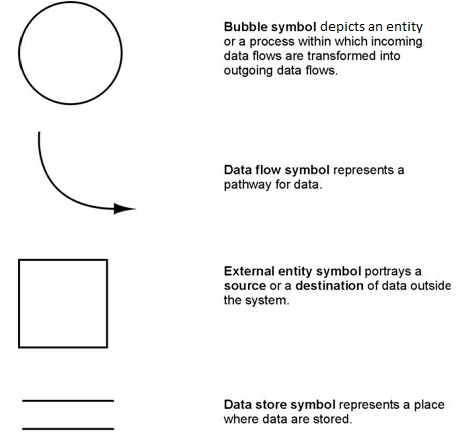
\includegraphics[scale=1]{dfd.png}
\caption{Notations used in  DFD}
\label{Notations used in  DFD}
\end{center}
\end{figure}
\end{itemize}
\newpage


\newpage
\subsection{Level 0 DFD}
Level 0 DFD gives a simple information about the overall structure. 
\begin{figure}[h!]
\begin{center}

\hspace{1 in}
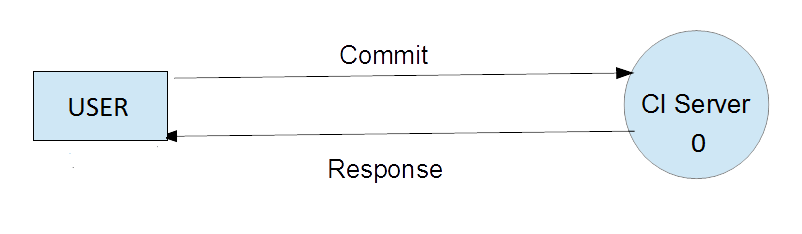
\epsfig{width=4in, file=dfd1.png}
\caption{Level 0 DFD}
\end{center}
\end{figure}

\subsection{Level 1 DFD}
The level 1 DFD gives a basic structure of the project indicating the five modules needed to execute the project.
\newpage
\begin{figure}[h]
\begin{center}
\hspace{1 in}
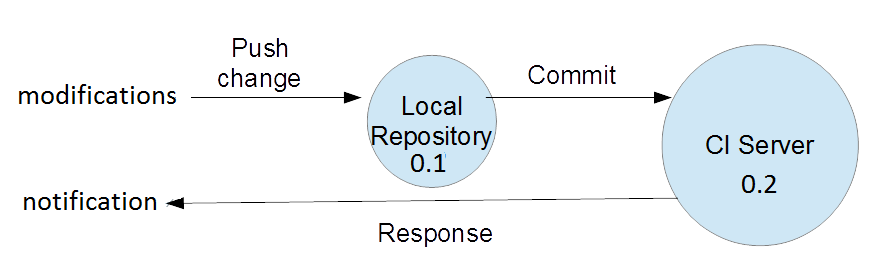
\epsfig{width=4in, file=dfd2.png}
\caption{Level 1.1 DFD}
\end{center}
\vspace{-1.5 in}
\end{figure}

%\begin{figure}[h]
%\begin{center}
%\epsfig{width=5in, file=dfd1_2.jpg}
%\caption{Level 1.1 DFD}
%\end{center}
%\end{figure}
\vspace{100pt}
\subsection{Level 2 DFD}
The level 2 DFD gives a much more advanced idea about the execution. Each of these sections perform unique functions and these are combined together to yield the final product.
\begin{figure}[h]
\begin{center}
\vspace{0.5 in}
\hspace{.0 in}
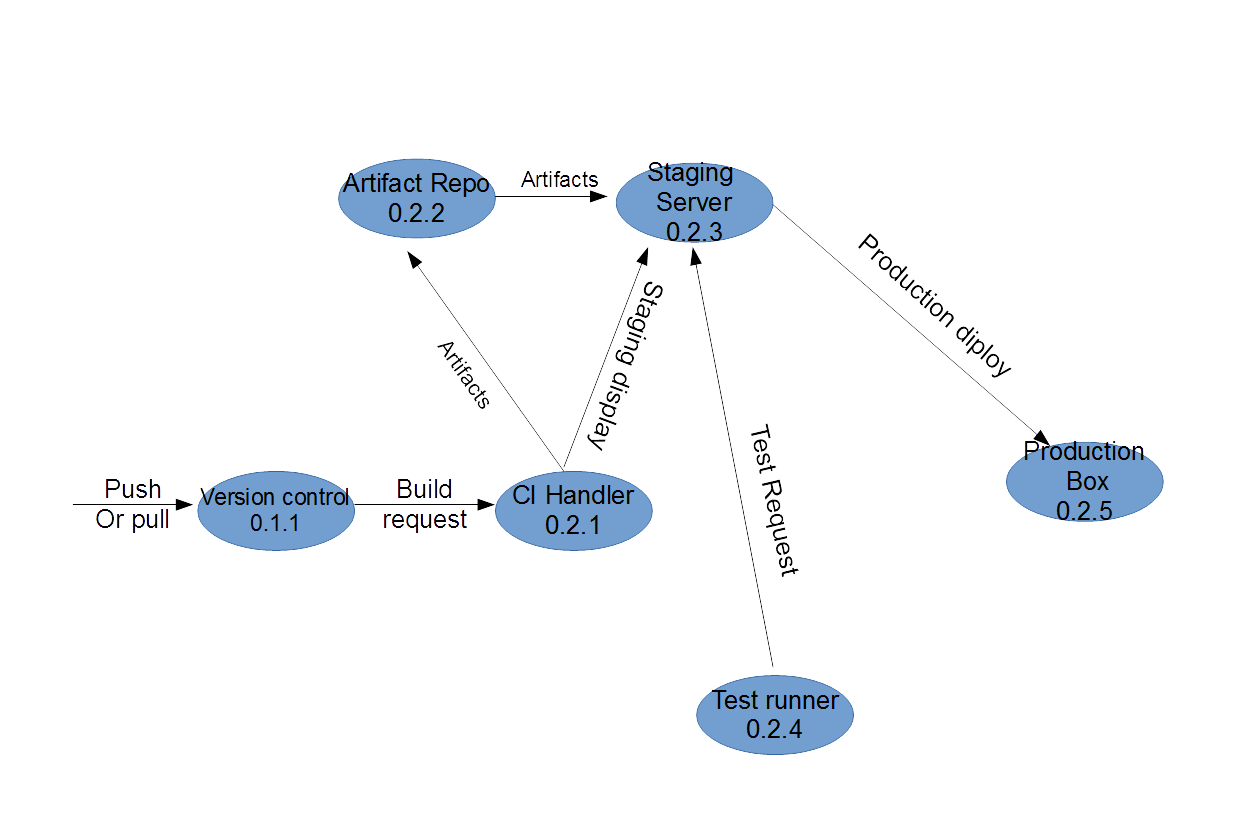
\epsfig{width=6in, file=dfd3.png}
\caption{Level 2.1.1 DFD}
\end{center}

\end{figure}
\pagebreak

\section{Flow Diagram}
\begin{figure}[h]
\begin{center}

\hspace{.0 in}
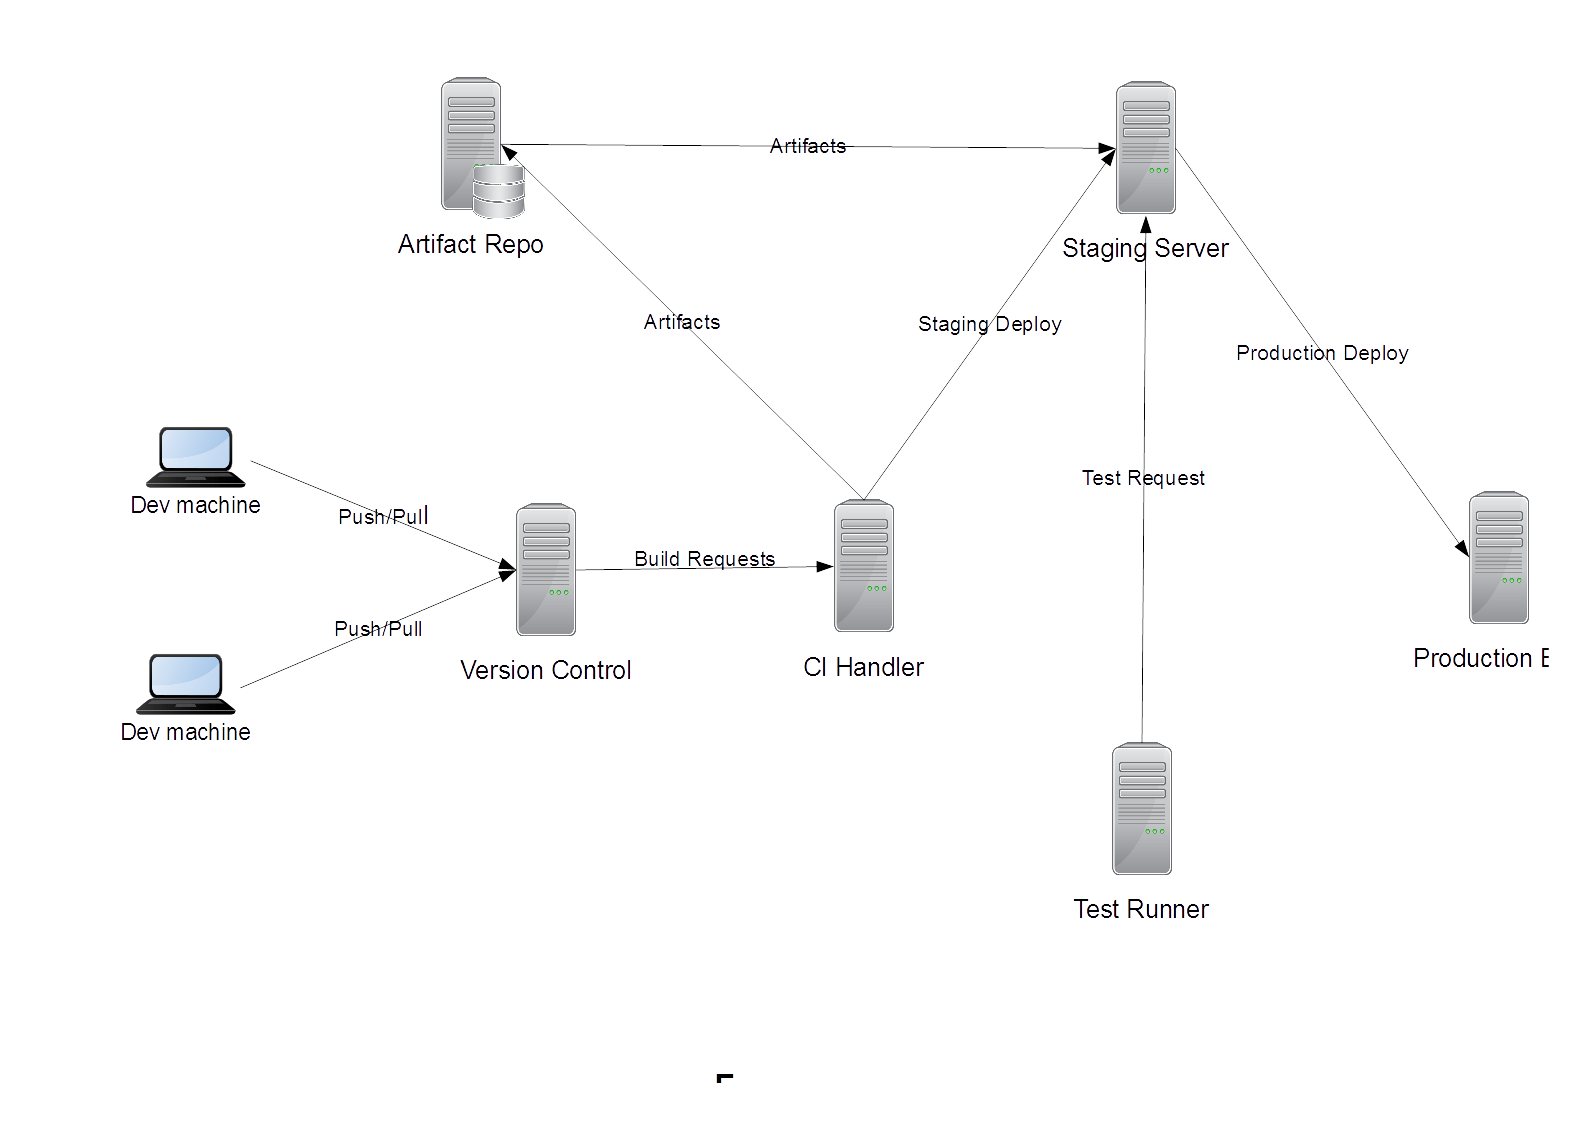
\epsfig{width=6in, file=flow1.png}
\caption{Flow diagram}
\end{center}

\end{figure}
\pagebreak
\section{C.I Pipeline Diagram}
\begin{figure}[h]
\begin{center}

\hspace{.0 in}
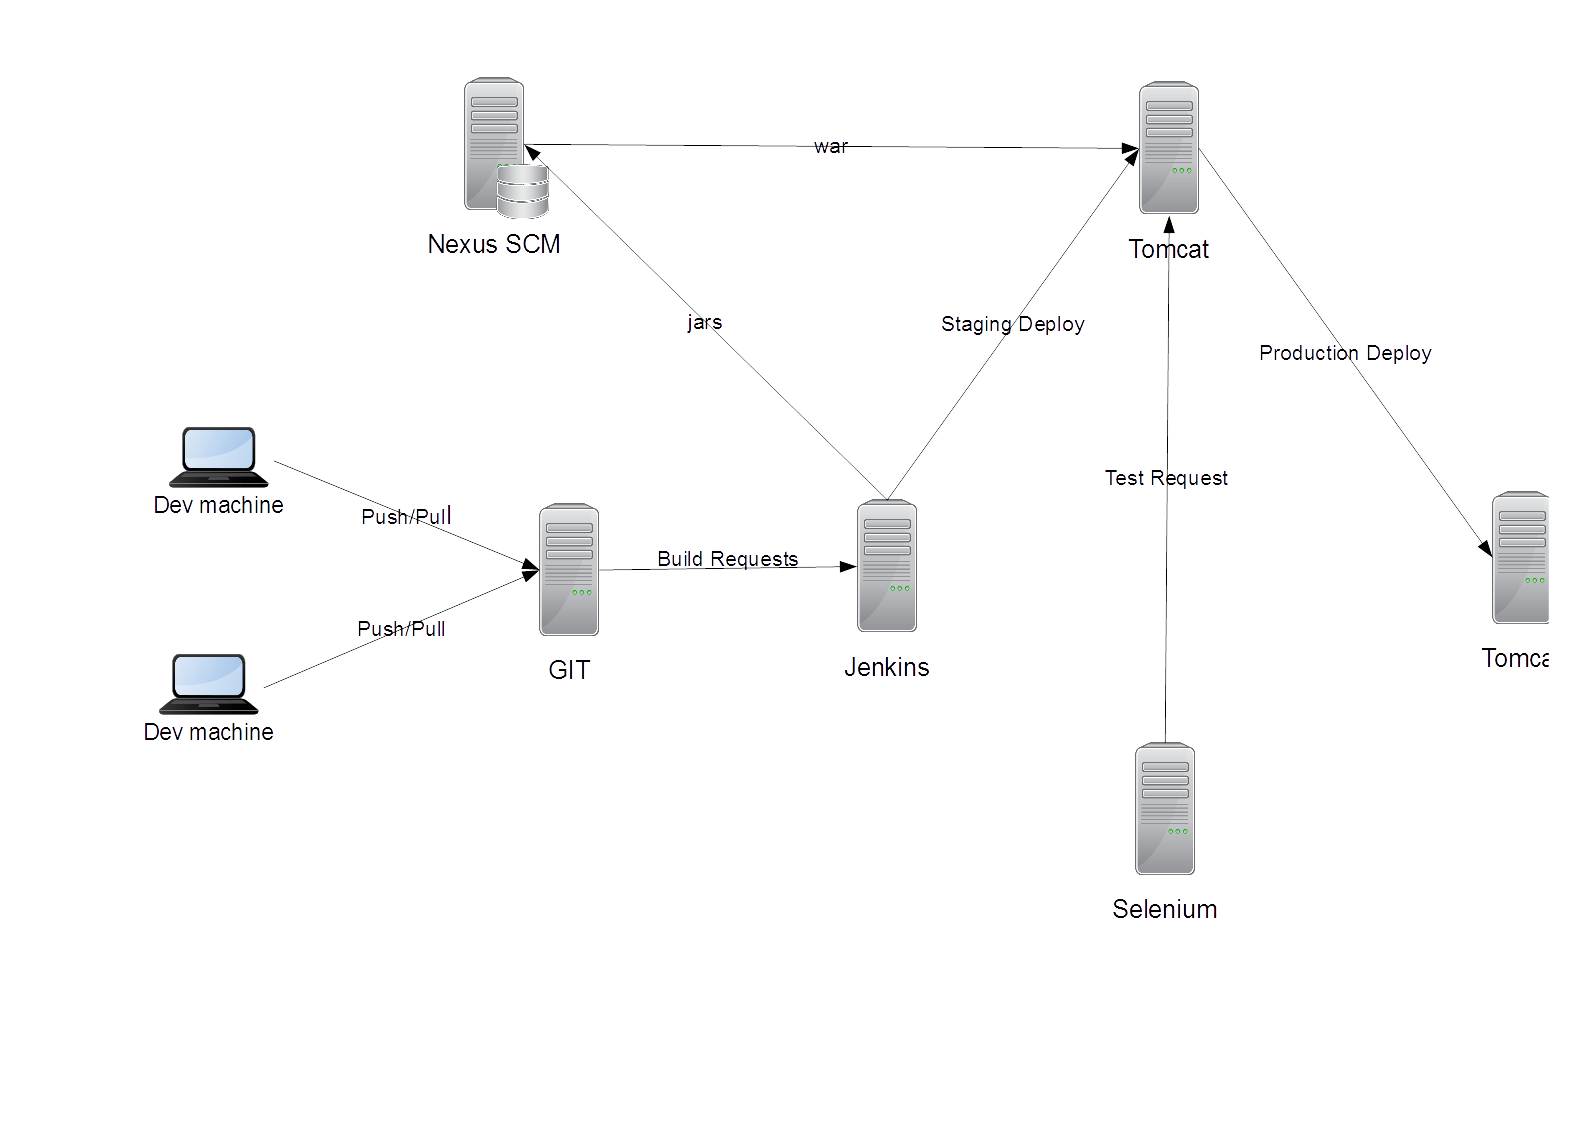
\epsfig{width=6in, file=pipeline.png}
\caption{C.I Pipeline}
\end{center}

\end{figure}
\pagebreak
\section{Sequence Diagram}
\par A Sequence diagram is an interaction diagram that shows how processes operate with
one another and in what order. It is a construct of a Message Sequence Chart. A sequence
diagram shows object interactions arranged in time sequence. It depicts the objects and classes
involved in the scenario and the sequence of messages exchanged between the objects needed
to carry out the functionality of the scenario.
\begin{figure}[h]
\begin{center}

\hspace{.0 in}
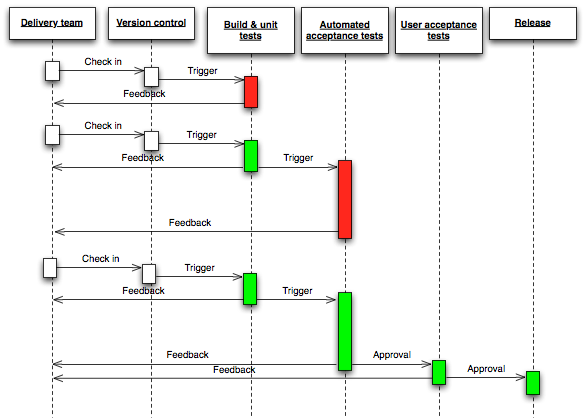
\epsfig{width=6in, file=sequence.png}
\caption{sequence}
\end{center}

\end{figure}


\chapter{IMPLEMENTATION}
Implementation is the stage in the project where the theoretical design is turned into a working system and is giving confidence about the new system to users that it will work effectively. It involves careful planning, investigation of the current system and it constraints on implementation, design of achieve the changeover, an evolution of change over method. The product is developed in Java environment in android platform. The software used for the development are Android Studio and SQLyog for the database. The hardware platform is Raspberry pi, collision sensor and arduino. This chapter may explain our implementation details.

\section{LANGUAGES AND PLATFORM USED}
\par The product is developed in Java environment and we are using SQLyog for database. SQLyog Server automatically tunes many of the server configuration options, therefore requiring little, if any, tuning by a system administrator. Although these configuration options can be modified by the system administrator, it is generally recommended that these options be left at their default values, allowing SQLyog Server to automatically tune itself based on run-time conditions.

\subsection{Python}
\par Python is a widely used high-level, general-purpose, interpreted, dynamic programming language. Its design philosophy emphasizes code readability, and its syntax allows programmers to express concepts in fewer lines of code than possible in languages such as C++ or Java. The language provides constructs intended to enable writing clear programs on both a small and large scale. Python supports multiple programming paradigms, including object-oriented, imperative and functional programming or procedural styles. It features a dynamic type system and automatic memory management and has a large and comprehensive standard library. Python interpreters are available for many operating systems, allowing Python code to run on a wide variety of systems. Python is managed by the non-profit Python Software Foundation.
\subsection{Android}
Android Studio is the official integrated development environment (IDE) for Android platform development. Android is a mobile operating system based on the Linux kernel and currently developed by Google. With a user interface based on direct manipulation. Android is designed primarily for touch screen mobile devices.\\
\subsection{Jsp}
\par Java Server Pages (JSP) is a server-side programming technology that enables the creation of dynamic, platform-independent method for building Web-based applications. A Java Server Pages component is a type of Java servlet that is designed to fulfill the role of a user interface.
JSP is a technology that helps software developers create dynamically generated web pages based on HTML, XML, or other document types. Released in 1999 by Sun-Microsystems, JSP is similar to PHP and ASP, but it uses the Java programming language. JSP tags can be used for a variety of purposes, such as retrieving information from a database or registering user preferences, accessing Java Beans components, passing control between pages and sharing information between requests.\\
\section{SCREEN SHOTS}
\subsection{Android Application}
\begin{itemize}
\item \par When a user installs SAVE ME in their mobile phone, a screen for app registration may appear of the following form. 
\begin{figure}[h]
\begin{center}
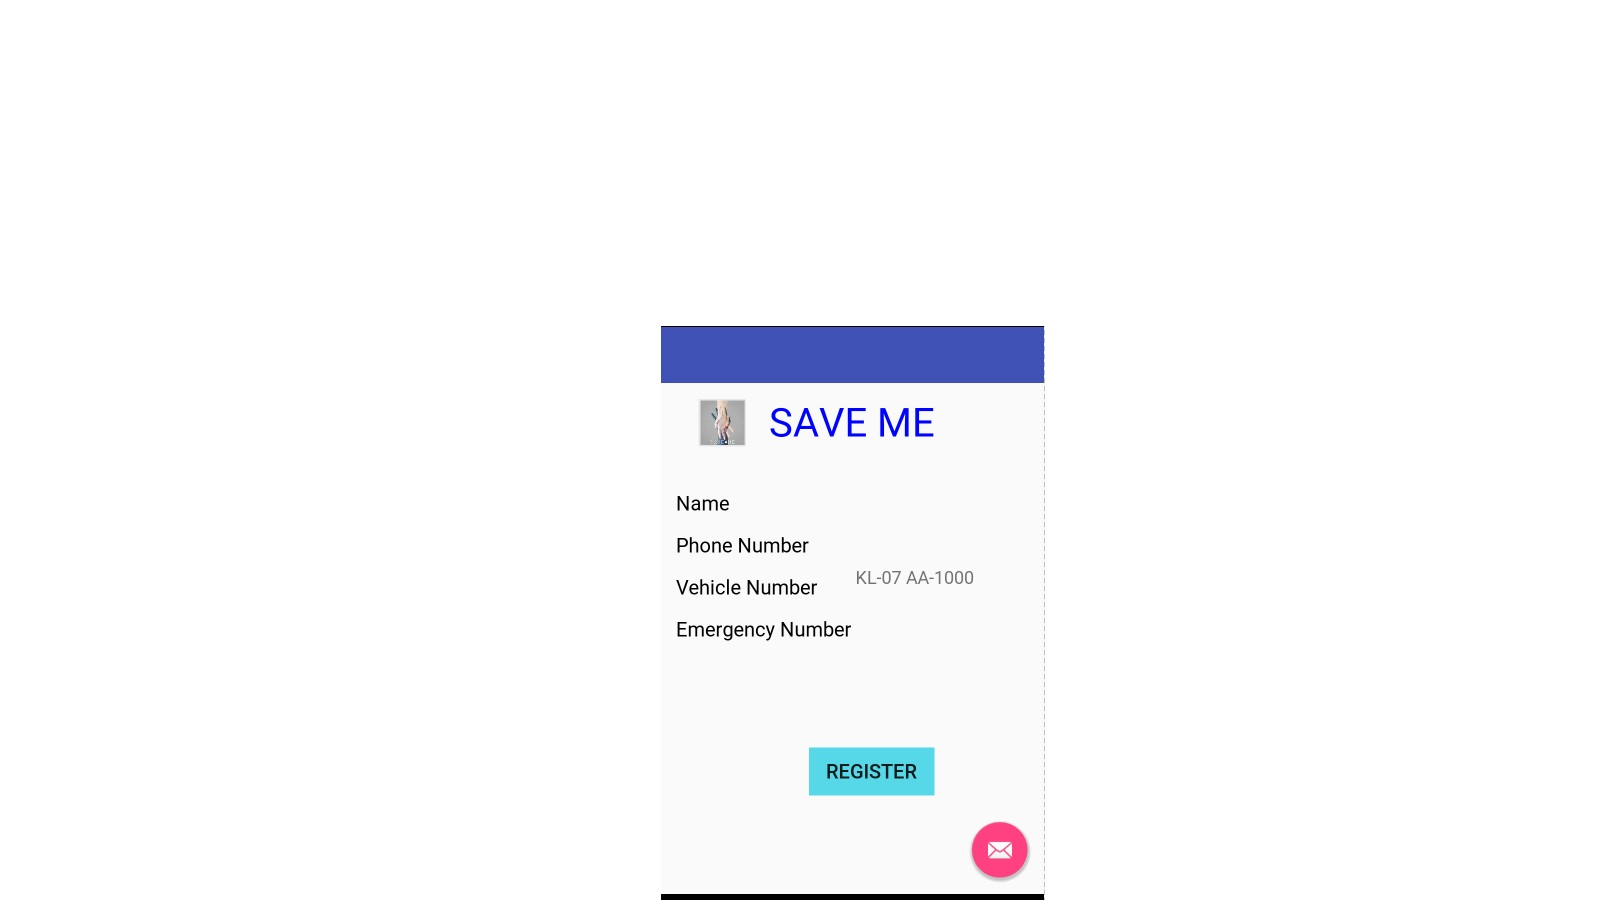
\includegraphics[scale=.4]{vehicalReg.jpg}
\caption{user registration in android application}
\label{user registration in android application}
\end{center}
\end{figure}
\newpage
\item \par Any user using the app has to press the connect button in order to establish connection with the server. A screen of the following format may appear.
\begin{figure}[h]
\begin{center}
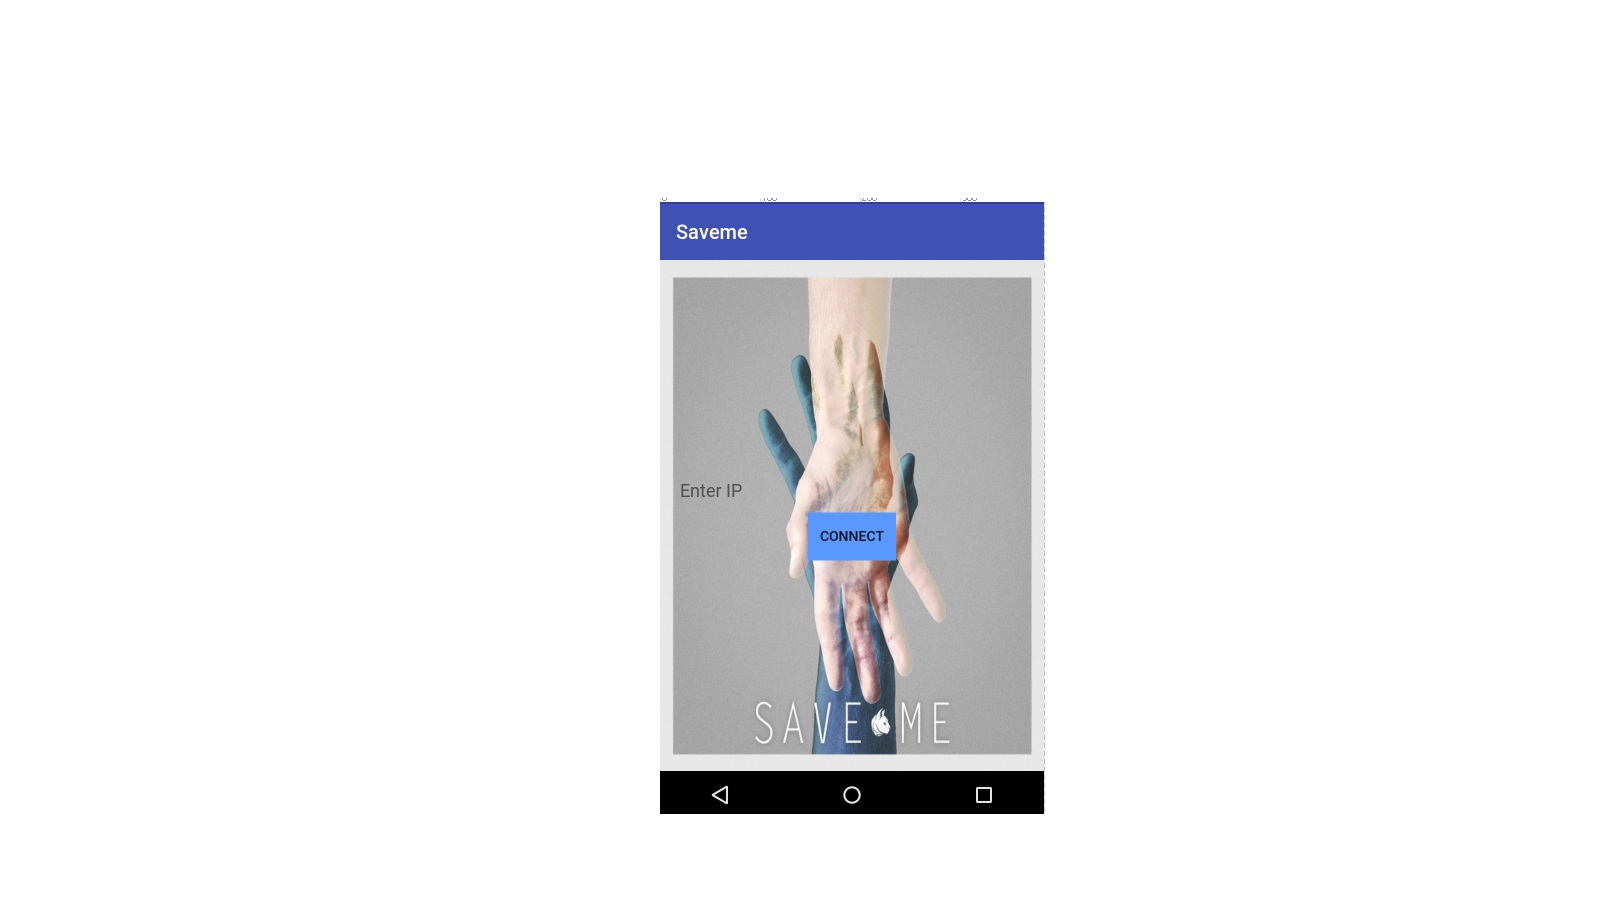
\includegraphics[scale=.4]{ipSeting.jpg}
\caption{Connecting to Server}
\label{Connecting to Server}
\end{center}
\end{figure}
\end{itemize}
\newpage 
\subsection{Web page}
\begin{itemize}

\item \par Whenever an accident occurs the server sends an accident notification to the near-by control station of the accident location.
\begin{figure}[h]
\begin{center}
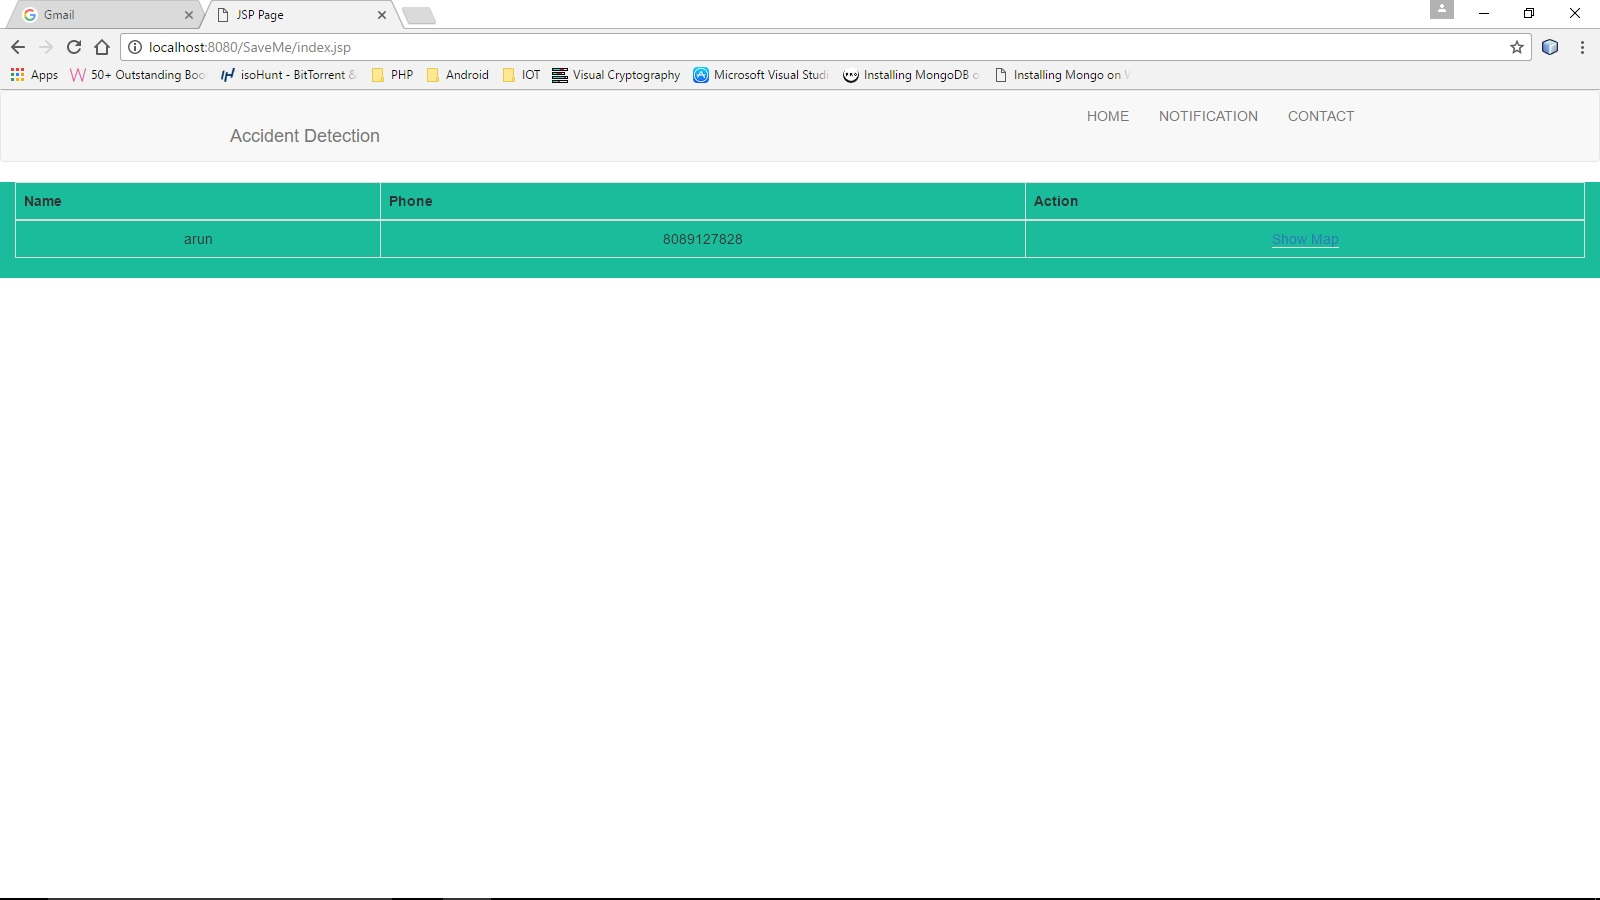
\includegraphics[scale=.4]{Notification.jpg}
\caption{Accident notification in web page}
\label{Accident notification in web page}
\end{center}
\end{figure}
\newpage
\item \par A map will appear with the indication of the accident area in the web page as in the following way for locating the exact location.

\begin{figure}[h]
\begin{center}
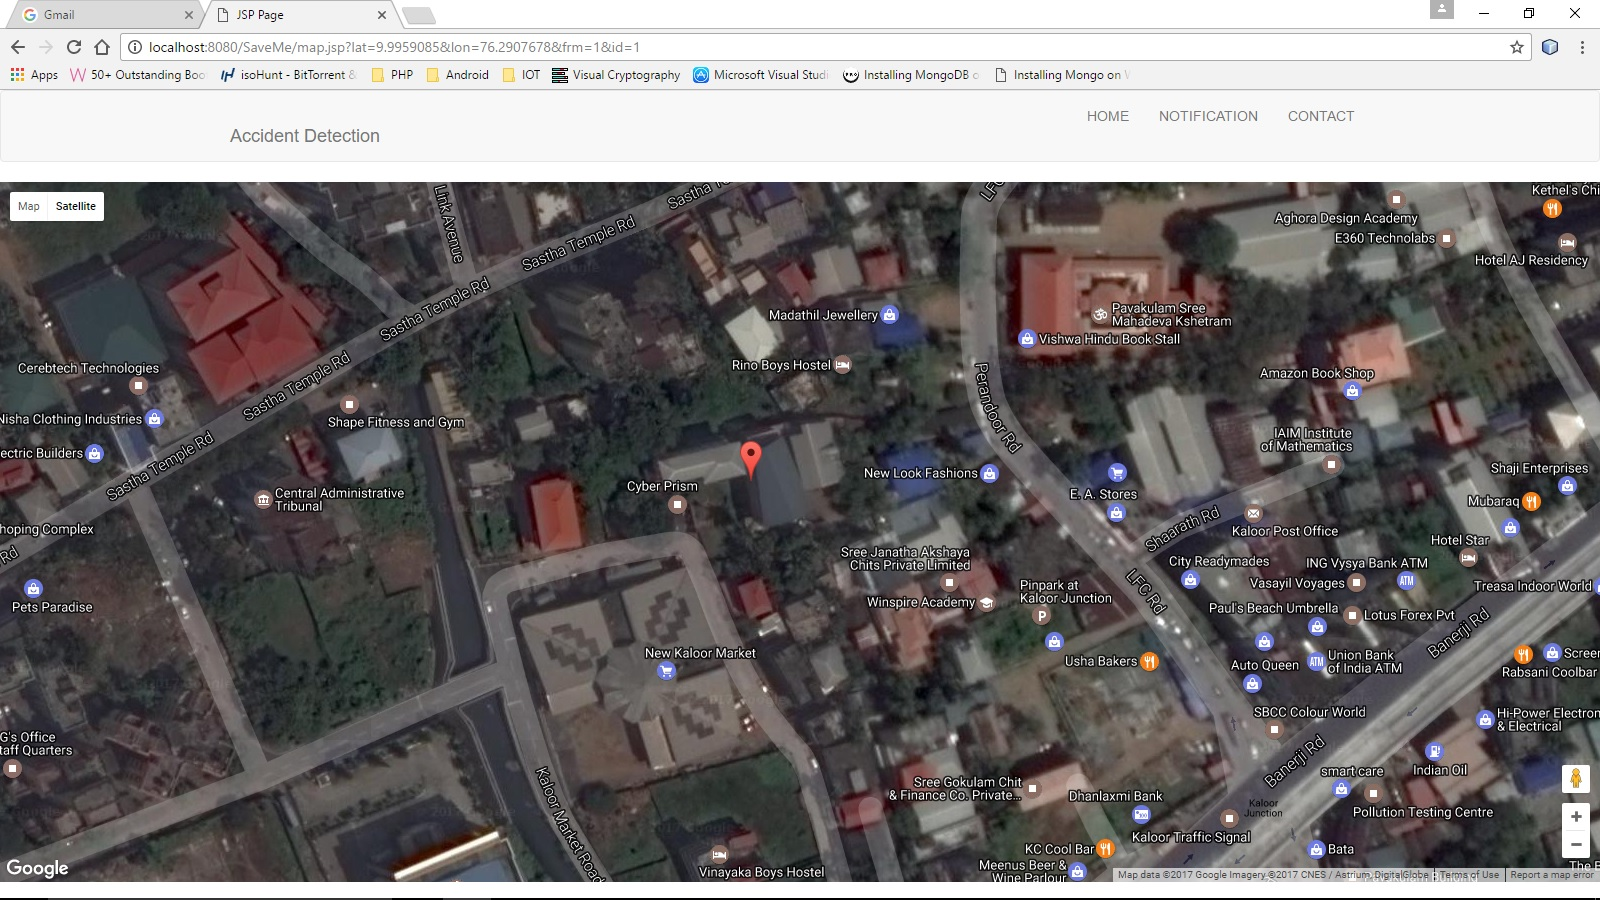
\includegraphics[scale=.4]{maps.jpg}
\caption{Map in web page}
\label{Map in web page }
\end{center}
\end{figure}
\end{itemize}
\chapter{TESTING}
\par When a system is developed, it is hoped that it performs properly. In practice, however some errors always occur. The main purpose of testing an information system is to find the error and correct them. A successful test is one that finds an error. System testing is a critical aspect of Software Quality Assurance and represents the ultimate review of specification, design and coding. Testing is the process of executing a program with the intent of finding an as yet undiscovered error. Nothing is complete without testing. Testing is vital to the success of the system.\\
\par The main objectives of the system testing are:\\
\begin{itemize}
\item To ensure during operation the system will perform as per specification. 
\item To make sure that the system meets user requirements during operation.
\item To verify that the controls incorporated in the system function as intended.
\end{itemize}
\par If the testing conducted successfully, it will uncover errors in the software. As a secondary benefit, testing demonstrates that the software functions appear to be working according to specification and that performance requirements appear to have been satisfied.\\
\par The system “Save Me” is tested in such a way that almost all errors that may occur are found and corrected. The test process carried out in this system includes the following:\\
\section{CODE TESTING}
\par In code testing the logic of the developed system is tested. For this every module of the program is executed to find any error. To perform specification test, the examination of the specifications stating what the program should do and how it should perform under various conditions.This testing was done side by side with coding. This examines the logic of the program. In Java special test cases are used for testing the code. Every part of the program was tested in this phase.

\section{UNIT TESTING}
\par Unit testing is undertaken after a module has been coded and reviewed. Before carrying this testing, the unit test cases have to be designed and the test environment for the unit under test has to be developed. The various test cases are driver and stub modules. The main objective is to determine the correct working of the individual modules. During the testing each module is isolated from other modules and individually unit tested. It involves a precise definition of the test cases, testing criteria, and management of test cases. The modules that are tested include \\
Android module, Server module and Sensing module.

\section{INTEGRATION TESTING}
\par System testing does not test the software as a whole, but rather than integration of each module in the system. The primary concern is the compatibility of individual modules. One has to find areas where modules have been designed with different specifications of data lengths, type and data element name. Testing and validation are the most important steps after the implementation of the developed system. The system testing is performed to ensure that there are no errors in the implemented system. The software must be executed several times in order to find out the errors in the different modules of the system. Each of the modules were integrated together and subjected to testing. \\
\section{VALIDATION TESTING}
\par Validation refers to the process of using the new software for the developed system in a live environment i.e., new software inside the organization, in order to find out the errors. The validation phase reveals the failures and the bugs in the developed system. It will come to know about the practical difficulties the system faces when operated in the true environment. Validation test was performed in the Login section. By testing the code of the implemented software, the logic of the program can be examined. A specification test is performed to check whether the specifications stating the program are performing under various conditions. Apart from these tests, there are some special tests conducted which are given below:
\begin{itemize}
\item Peak load test This determines whether the new system will handle the volume of activities when the system is at the peak of its processing demand. The test has revealed that the new system is capable of handling the demands at the peak time.
\item Storage testing This determines the capacity of the new system to store transaction data on a disk or on other files. The proposed software has the required storage space
available.
\item Performance time testing This test determines the length of the time used by the system to process transaction data.
\end{itemize}
\section{SYSTEM TESTING}
\par After all units of a program have been integrated together and tested, system testing is taken up. It is same for both procedural and object oriented programming. System tests are designed to validate a fully developed system to assure that it meets its requirements. The system test cases can be classified into performance and functionality test cases. The functionality test cases are designed to check whether the software satisfies the functional requirements as documented in the SRS document. The performance tests on the other hand test the conformance of the system with non-functional requirements of the system.\\
\section{OUTPUT TESTING}
\par After the performance of unit testing, the next step is output testing. No system would be useful if it does not produce the required output in the specific format, thus output format on the screen is found to be correct when the format was designed in the system phase according to the user need.\\
\par The maintenance of software is the time period in which software product performs useful works. Maintenance activities involve making enhancement to software product, adapting product to new environment and correcting problems. It includes both the improvement of the system function.
\par It may involve the continuing involvement of a large proportion of computer department resources. The main task may be to adapt existing system in a changing environment. System should not be changed casually following informal requests. To avoid unauthorized amendments, all requests for change should be channeled to a person nominated by management. The nominated person has sufficient knowledge of the organizations computer based systems to be able to judge the relevance of each proposed change.
\par No annual costs for support or maintenance are required. Of course, the individual system components come with limited warranty from the manufacturers, eg:, the PC, mobile phones, etc.
\par There is no obligation to purchase or pay for any extended maintenance or support.
\section{GOAL OF TESTING}
\par Many users may use our project. So the project designer must test all the modules of the project. The main goal of our project is, whenever user uses our project, it should run without any error.
\section{PASS/FAIL CRITERIA}
The pass/fail criteria specifies a set of constraints whose satisfaction leads to approval or disapproval of the proper functioning of the system .
\section{PASS CRITERIA}
\par The system must meet all the functional and non-functional requirements. Pass all the test cases, get the expected response, and get acceptable performance to be tested pass.
\begin{itemize}
\item	User can login and submit request.
\item	Officials can verify and process the request
\item	Periodic update of database
\end{itemize}
\section{FAIL CRITERIA}
\par If one of the following situations happens, the system is considered to fail:
\begin{itemize}
\item	User cannot login
\item	Database updation failure
\item	OTP sending failed
\item	Human error
\end{itemize}
\section{TEST REPORTS}
The detailed test reports prepared for each function. A sample test report is given below:
\begin{table}[!htb]
\centering
\caption{Test Report}
\label{Test Report}
\begin{tabular}{|l|l|}
\hline
Name                                                                                & SAVE ME                                              \\ \hline
Version                                                                             & 1.0                                                                  \\ \hline
Author                                                                              & Anamika G V, Mekha S, Priyanka S, Safeena Ashraf.              \\ \hline
Approved By                                                                         & Self                                                                 \\ \hline
Date                                                                                & Monday, 6th March 2017                                            \\ \hline
Role                                                                                & User can operate the system.                                          \\ \hline
Prerequisite                                                                        & The user is logged into the system                                   \\ \hline
User/Actor                                                                          & System Response                                                      \\ \hline
Registration                                                                        & User can register and use the system.                 \\ \hline
Run Applications                                                                    & Any accident may be detected and notification
 may be reported. \\ \hline
Handle User Data                                                                    &The server can handle various user data                                                                      \\ \hline
                                                                                    
\begin{tabular}
[c]{@{}l@{}}The test project\\ was successfully\\ saved
\end{tabular} 
&                                                                      \\ \hline
\end{tabular}
\end{table}
\par Test case preparation helps the user and the developer to find and fix the errors easily and in advance. Save Me is well tested with the proper test cases and thus passed a better unit test. Elaborated test cases also prepared subjected the system for thorough testing. The test cases prepared are in the above format.
\section{BLACK BOX TESTING}
\par Black-box testing is a method of software testing that examines the functionality of an application without peering into its internal structures or workings. Test case preparation helps the user and the developer to find and fix the errors easily and in advance. 
\par The test cases prepared are in the following format:
\begin{table}[!htb]
\centering
\caption{Test Cases}
\label{Test Cases}
\begin{tabular}{|l|l|l|l|l|l|}
\hline
Test & Usecase step & \begin{tabular}[c]{@{}l@{}}Action performed\\ /User input\end{tabular} & \begin{tabular}[c]{@{}l@{}}Expected Result\\ /system response\end{tabular} & \begin{tabular}[c]{@{}l@{}}Actual          \\    result\end{tabular} & \begin{tabular}[c]{@{}l@{}}Do expected \\and  actual \\result \\correspond\end{tabular} \\ \hline
1   & Admin          & \begin{tabular}[c]{@{}l@{}}Create user\end{tabular}         & \begin{tabular}[c]{@{}l@{}}Successful	creation\\ of user\end{tabular}                 & As Expected                                                          & Yes                                                    \\ \hline
2   & User                                                                       & \begin{tabular}[c]{@{}l@{}}Enter name \\phone no.\\ emergency no. \\ vehicle no.\end{tabular}   		& \begin{tabular}[c]{@{}l@{}}Display success.\\
Next page \\ contain a \\ connect button 
\end{tabular}              & As Expected                                                          & Yes                                                                                     \\ \hline
3     & User         & \begin{tabular}[c]{@{}l@{}}Presses the\\ connect button\end{tabular} & \begin{tabular}[c]{@{}l@{}}Connection\\ establish \\ between user \\and raspberry pi\end{tabular}                 & As Expected                                                          & Yes                                                                                                                      \\ \hline
4     & Sensor         & \begin{tabular}[c]{@{}l@{}}Crack in\\ sensor
when\\ accident occurs
\end{tabular} & \begin{tabular}[c]{@{}l@{}}arduino converts\\ analog signal\\ to digital\\ and send to pi\end{tabular}                 & As Expected                                                          & Yes                                                                                     \\ \hline
5     & Sensor         & \begin{tabular}[c]{@{}l@{}}Pi sense\\ threshold \\and send\\ to phone\end{tabular} & \begin{tabular}[c]{@{}l@{}}Get \\notification\\ in phone\\ page\end{tabular}                 & As Expected                                                          & Yes 			\\  \hline
6     & User         & \begin{tabular}[c]{@{}l@{}}Send \\accident\\ information\\ to control\\ station and \\emergency no. \end{tabular} & \begin{tabular}[c]{@{}l@{}}Get location\\ of accident\\ and take \\rescue \\action\end{tabular}                 & As Expected                                                          & Yes           \\ \hline
\end{tabular}
\end{table}

\chapter{FUTURE SCOPE}
\par In the proposed system all details about the system is designed into an application. SAVE ME: An Automatic Accident Detection And Alert System For Automobiles is used for providing help to the accident victims. There are many cases where valuable lives are lost due to the lack of help at the correct time. We are developing this application for providing help in case of accidents for the victims.It is designed as a web based application, which will work smoothly on any computer system with internet connection. The application sends the accident message to the nearest control station as well as to the emergency number provided by the application user. The application provides the exact GPS location of the accident site which makes it very helpful for the police to provide immediate help for the victim. The document automation software is also supported by a powerful database where the documents are arranged, making updates and collaboration easy and fast. The system proposed here is meant for use in any automobile with the user having android mobile phone. The basic steps in application processing is same everywhere, and hence the extended version of this system can be used in advanced areas too. 
\chapter{CONCLUSION}
\par SAVE ME: An Automatic Accident Detection And
Alert System For Automobiles is used for providing help to the accident victims. There are many cases where valuable lives are lost due to the lack of help at the correct time. We are developing this app for providing help in case of accidents for the victims. The app sends the accident message to the the nearest control station as well as to the emergency number provided by the app user. The app provides the exact GPS location of the accident site which makes it very helpful for the police to provide immediate help for the victim. With the help of this app we may be able to save many lives as there is sureity of help.
\renewcommand{\bibname}{\uppercase{REFERENCES}}
\begin{thebibliography}{999}
\addcontentsline{toc}{chapter}{7\hspace{0.1in} REFERENCES}


\bibitem{r1} Bhandari Prachi, Dalvi Kasturi, Chopade Priyanka,\quotes{ Intelligent Accident-Detection And Ambulance- Rescue System} \textit{INTERNATIONAL JOURNAL OF SCIENTIFIC and TECHNOLOGY RESEARCH}, VOLUME 3, ISSUE 6, JUNE 2014
\bibitem{r2} Collision avoidance system.Dec.2013.[Online].Available:https://en.wikipedia.org/ wiki/Collision/avoidance/system.
\bibitem{r3} Raspberry pi,Sept.2013.[Online]. Available:https://en.wikipedia.org/wiki/Raspberry/Pi.




\end{thebibliography}
\chapter*{GLOSSARY}
\textbf{ER}  : Entity Relationship
\par \textbf{GPS} : Global Positioning System
 \par \textbf{HTTP} : Hyper Text Transfer Protocol
\par \textbf{IPV4} : Internet Protocol Version 4
\par  \textbf{JSP} : Java Server Page
\par \textbf{SQL} : Structured Query Language
\par \textbf{UML} : Unified Modeling Language
\par \textbf{ERD} : Entity Relationshi Diagram
\par \textbf{JVM} : Java Virtual Machine
\par \textbf{DFD} : Data Flow Diagram
%\end{document}

\begin{theindex}

\addcontentsline{toc}{chapter}{\hspace{0.5cm} INDEX}
\rhead{\empty}
\lhead{\empty}
\lfoot{\empty}
%\hspace{.1in}
\vspace{.2in}
\large\textbf{A}
\item  Android 
\item  Android Application, 1
\item Arduino , 7

\vspace{.2in}
\large\textbf{C}
\item Conclusion , 14

\vspace{.2in}
\large\textbf{D}
\item Data Flow Diagram , 8
\item Database, 11
\item Design, 7
\vspace{.2in}
\large\textbf{E}
\item ER Diagram , 16
\item Existing system, 
\vspace{.2in}

\large\textbf{F}
\item Functional Requirements , 16
\vspace{.2in}

\large\textbf{G}
\item Gantt chart , 16
\item Goal of testing, 
\vspace{.2in}

\large\textbf{H}
\item Hardware Requirements , 8

\vspace{.2in}
\large\textbf{I}
\item Introduction , 1
\item Integration Testing

\vspace{.2in}
\large\textbf{J}
\item Java
\item  JSP
\vspace{.2in}
\large\textbf{M}
\item Modules , 4

\vspace{.2in}
\large\textbf{N}
\item Non Functional Requirements , 5

\vspace{.2in}
\large\textbf{O}
\item Operational Feasibility,8 
\item Output Testing

\vspace{.2in}
\large\textbf{P}
\item Python

\vspace{.2in}
\large\textbf{R}
\item References

\vspace{.2in}
\large\textbf{S}
\item Screen shots
\item Sequence Diagram
\item Software Requirements,12
\item System testing,67 

\vspace{.2in}
\large\textbf{T}
\item Technical Feasibility,8
\item Test reports

\vspace{.2in}
\large\textbf{U}
\item UML diagrams, 23 ,16
\item Use case diagram
\item  Unit Testing

\vspace{.2in}
\large\textbf{V}
\item Validation Testing

%\hspace{.6in}\large W

%\small

%\item wireless sensor, 1

%\item working period, 4\\


\end{theindex}

\end{document}

%\end{document}
